\section{Introduction}
\FloatBarrier % Now figures cannot float above section title

Our product is a type of mechanical equipment used for automated welding. Our robotic arm can be widely used in various welding operations in the manufacturing industry, including automotive manufacturing, aerospace, construction, and manufacturing.

Our product has many adavantages. Firstly, it can improve production efficiency and quality by reducing the negative impact of human factors on production through automated welding operations. Secondly, it can reduce the danger of the work environment. 

In summary, the four-arm welding robot is an efficient and accurate welding device with many advantages. It will become an important part of automated production in the manufacturing industry, providing a reliable solution for various production operations.









\iffalse
The purpose of this experiment is to investigate the behaviour of a mild steel portal frame model when subjected to increasing loads.

The rig consists of a loading system that applies a vertical load at the center of the beam and a horizontal load at the top of one column. As shown in \autoref{f0}.

\begin{figure}[htbp]
    \centering
    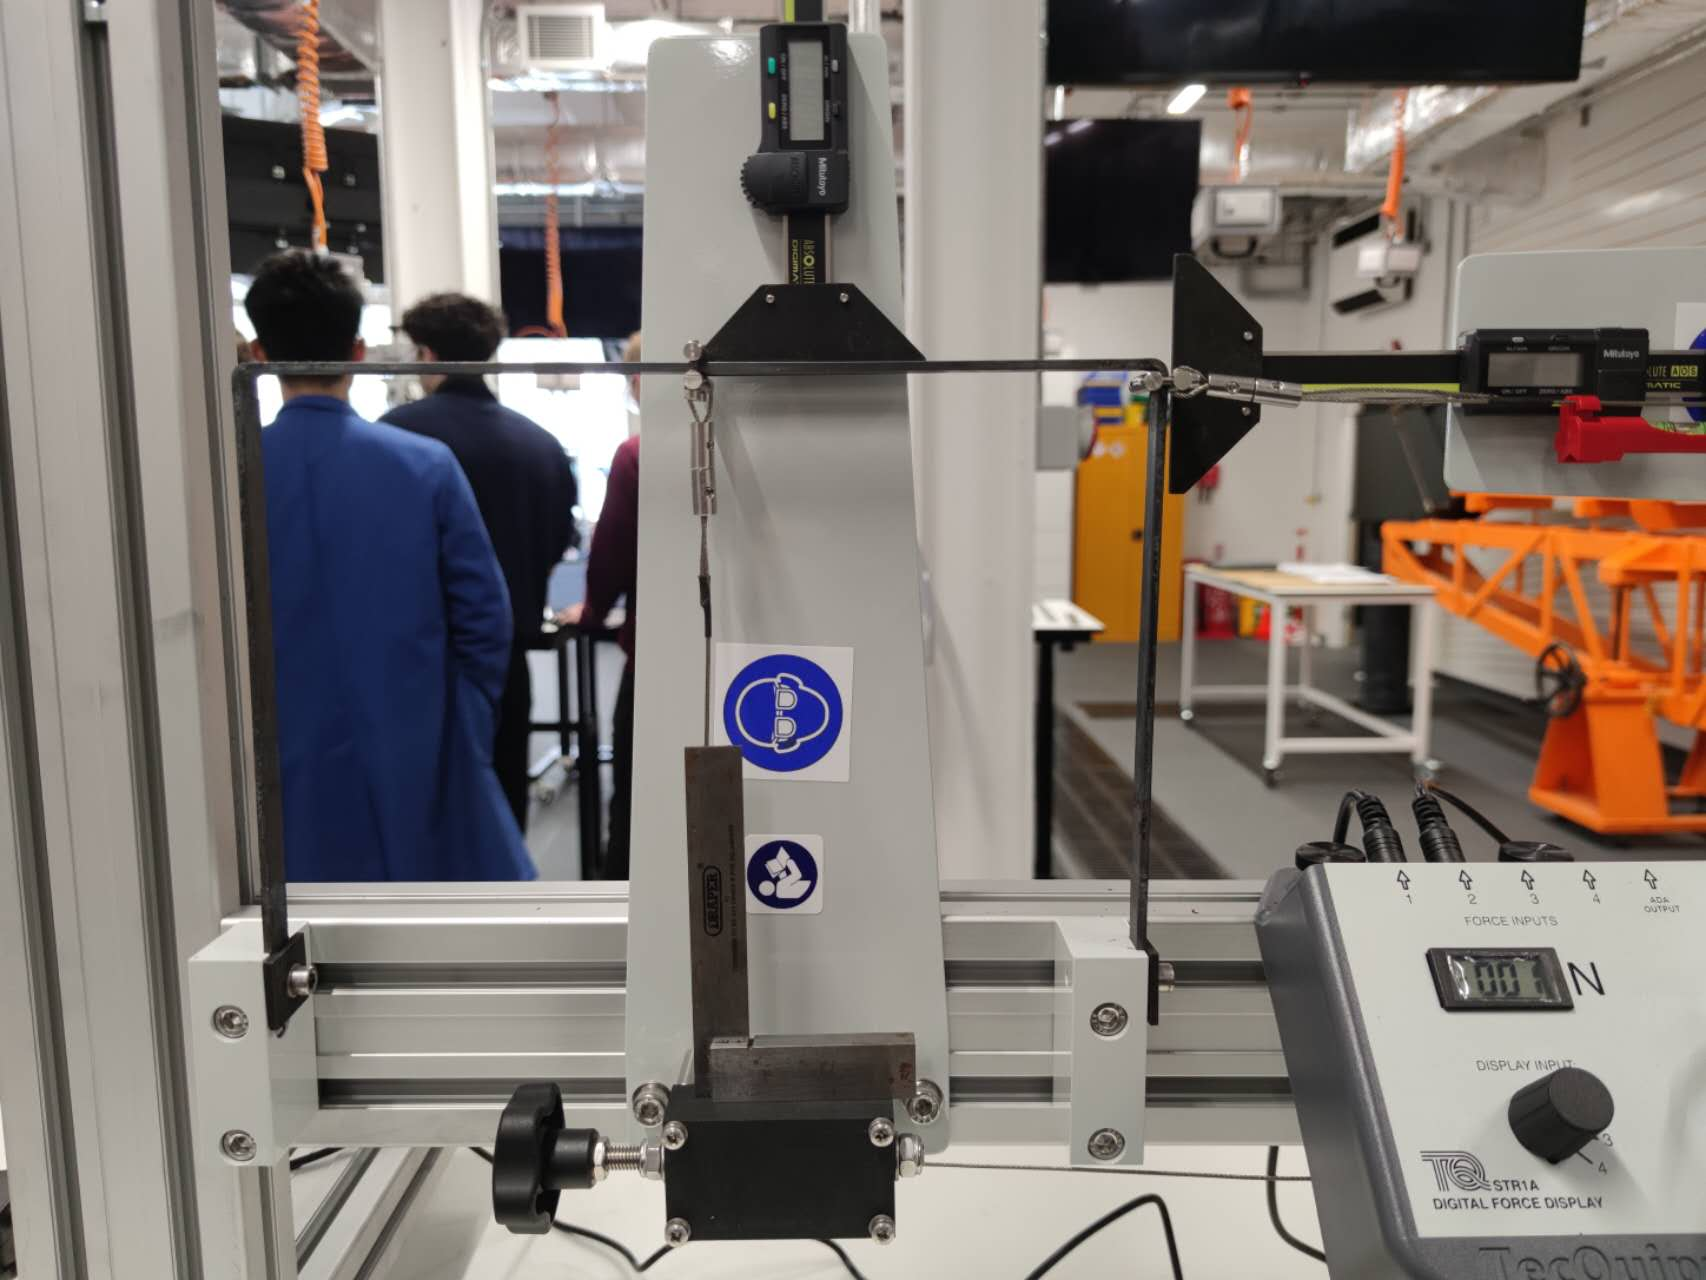
\includegraphics[width=7.5cm]{./fig/00.jpg}
    \caption{Experimental procedure}
    \label{f0}
\end{figure}

\fi


